\chapter{First Project}
\label{sec-crystals}


\begin{figure}[!h]
	\centering
	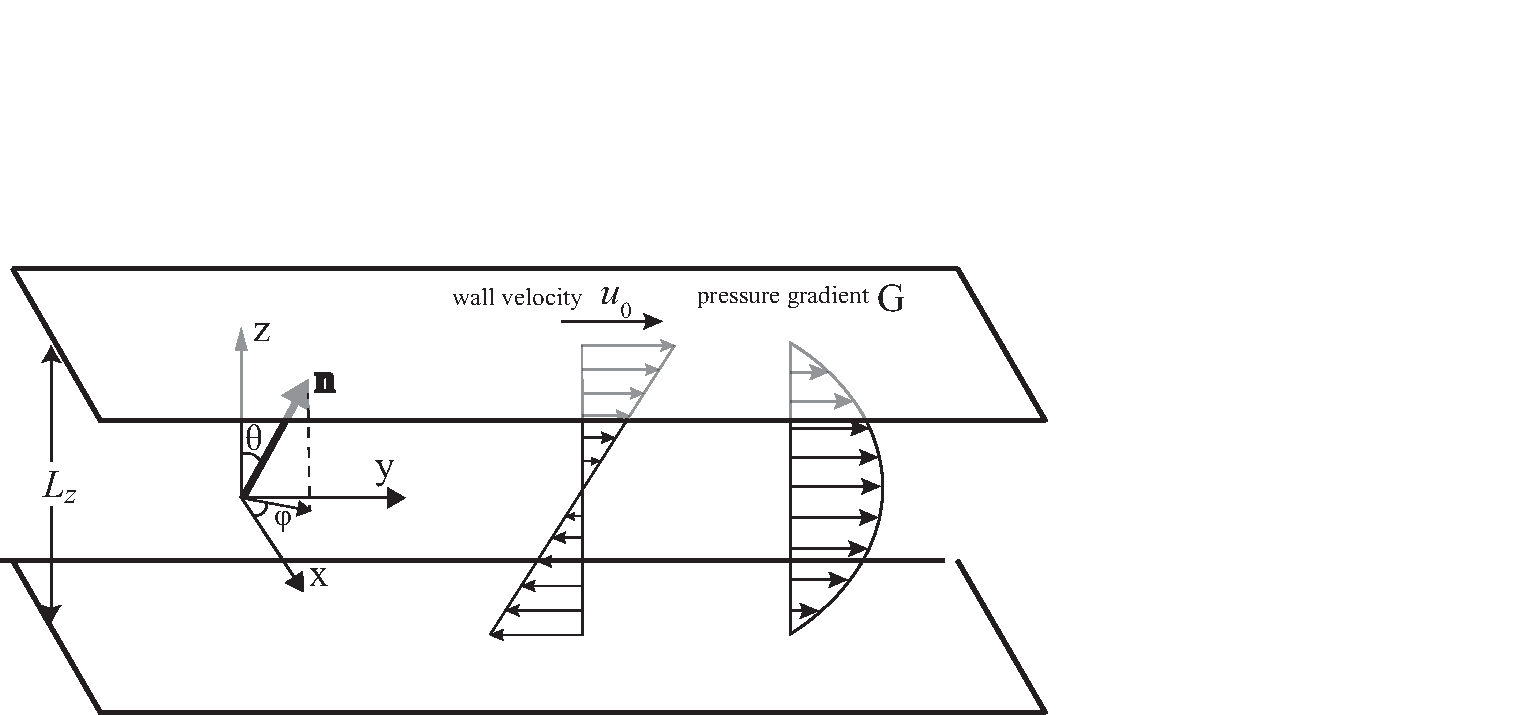
\includegraphics[width=1.0\linewidth]{images/Result1/figure1_setup.pdf}
	\caption{ {\bf Simulation setup.} Two walls are in $z$-direction separated by a distance of \emph{$L_z$}. Easy axis is in the $y$-direction. Couette flow is imposed by moving top and bottom wall in $y$-direction with speed $u_0$ and $-u_0$, respectively. Poiseuille flow is imposed by applying a pressure gradient \emph{$G$} along $y$-direction. Director field ${\bf n}$ is represented by a polar angle $\theta$ and an azimuthal angle $\phi$.}
	\label{fig2:setup}
\end{figure}


In this study, we conduct all the simulation in this flat channel Fig.~\ref{fig2:setup}. 


\section{Results-1st section}


\newpage
\section{Results-2nd section}

\newpage
\section{Conclusion}

-{\it Your conclusion of 1st project goes here}


\newpage

\section{Appendix}
\label{sec.appen}

\subsection{1st part of Appendix}
\label{appen_Leslie}